\documentclass[a4paper]{article}
\usepackage[a4paper, margin=1in]{geometry}
% Some basic packages
\usepackage[utf8]{inputenc}
\usepackage[T1]{fontenc}
\usepackage{textcomp}
\usepackage[dutch]{babel}
\usepackage{url}
\usepackage{graphicx}
\usepackage{float}
\usepackage{booktabs}
\usepackage{enumitem}

\pdfminorversion=7

% Don't indent paragraphs, leave some space between them
\usepackage{parskip}

% Hide page number when page is empty
\usepackage{emptypage}
\usepackage{subcaption}
\usepackage{multicol}
\usepackage{xcolor}

% Other font I sometimes use.
% \usepackage{cmbright}

% Math stuff
\usepackage{amsmath, amsfonts, mathtools, amsthm, amssymb}
% Fancy script capitals
\usepackage{mathrsfs}
\usepackage{cancel}
% Bold math
\usepackage{bm}
% Some shortcuts
\newcommand\N{\ensuremath{\mathbb{N}}}
\newcommand\R{\ensuremath{\mathbb{R}}}
\newcommand\Z{\ensuremath{\mathbb{Z}}}
\renewcommand\O{\ensuremath{\emptyset}}
\newcommand\Q{\ensuremath{\mathbb{Q}}}
\newcommand\C{\ensuremath{\mathbb{C}}}

% Easily typeset systems of equations (French package)
\usepackage{systeme}

% Put x \to \infty below \lim
\let\svlim\lim\def\lim{\svlim\limits}

%Make implies and impliedby shorter
\let\implies\Rightarrow
\let\impliedby\Leftarrow
\let\iff\Leftrightarrow
\let\epsilon\varepsilon

% Add \contra symbol to denote contradiction
\usepackage{stmaryrd} % for \lightning
\newcommand\contra{\scalebox{1.5}{$\lightning$}}

% \let\phi\varphi

% Command for short corrections
% Usage: 1+1=\correct{3}{2}

\definecolor{correct}{HTML}{009900}
\newcommand\correct[2]{\ensuremath{\:}{\color{red}{#1}}\ensuremath{\to }{\color{correct}{#2}}\ensuremath{\:}}
\newcommand\green[1]{{\color{correct}{#1}}}

% horizontal rule
\newcommand\hr{
    \noindent\rule[0.5ex]{\linewidth}{0.5pt}
}

% hide parts
\newcommand\hide[1]{}

% si unitx
\usepackage{siunitx}
\sisetup{locale = FR}

% Environments
\makeatother
% For box around Definition, Theorem, \ldots
\usepackage{mdframed}
\mdfsetup{skipabove=1em,skipbelow=0em}
\theoremstyle{definition}
\newmdtheoremenv[nobreak=true]{definitie}{Definitie}
\newmdtheoremenv[nobreak=true]{eigenschap}{Eigenschap}
\newmdtheoremenv[nobreak=true]{gevolg}{Gevolg}
\newmdtheoremenv[nobreak=true]{lemma}{Lemma}
\newmdtheoremenv[nobreak=true]{propositie}{Propositie}
\newmdtheoremenv[nobreak=true]{stelling}{Stelling}
\newmdtheoremenv[nobreak=true]{wet}{Wet}
\newmdtheoremenv[nobreak=true]{postulaat}{Postulaat}
\newmdtheoremenv{conclusie}{Conclusie}
\newmdtheoremenv{toemaatje}{Toemaatje}
\newmdtheoremenv{vermoeden}{Vermoeden}
\newtheorem*{herhaling}{Herhaling}
\newtheorem*{intermezzo}{Intermezzo}
\newtheorem*{notatie}{Notatie}
\newtheorem*{observatie}{Observatie}
\newtheorem*{oef}{Oefening}
\newtheorem*{opmerking}{Opmerking}
\newtheorem*{praktisch}{Praktisch}
\newtheorem*{probleem}{Probleem}
\newtheorem*{terminologie}{Terminologie}
\newtheorem*{toepassing}{Toepassing}
\newtheorem*{uovt}{UOVT}
\newtheorem*{vb}{Voorbeeld}
\newtheorem*{vraag}{Vraag}

\newmdtheoremenv[nobreak=true]{definition}{Definition}
\newtheorem*{eg}{Example}
\newtheorem*{notation}{Notation}
\newtheorem*{previouslyseen}{As previously seen}
\newtheorem*{remark}{Remark}
\newtheorem*{note}{Note}
\newtheorem*{problem}{Problem}
\newtheorem*{observe}{Observe}
\newtheorem*{property}{Property}
\newtheorem*{intuition}{Intuition}
\newmdtheoremenv[nobreak=true]{prop}{Proposition}
\newmdtheoremenv[nobreak=true]{theorem}{Theorem}
\newmdtheoremenv[nobreak=true]{corollary}{Corollary}

% End example and intermezzo environments with a small diamond (just like proof
% environments end with a small square)
\usepackage{etoolbox}
\AtEndEnvironment{vb}{\null\hfill$\diamond$}%
\AtEndEnvironment{intermezzo}{\null\hfill$\diamond$}%
% \AtEndEnvironment{opmerking}{\null\hfill$\diamond$}%

% Fix some spacing
% http://tex.stackexchange.com/questions/22119/how-can-i-change-the-spacing-before-theorems-with-amsthm
\makeatletter
\def\thm@space@setup{%
  \thm@preskip=\parskip \thm@postskip=0pt
}


% Exercise 
% Usage:
% \oefening{5}
% \suboefening{1}
% \suboefening{2}
% \suboefening{3}
% gives
% Oefening 5
%   Oefening 5.1
%   Oefening 5.2
%   Oefening 5.3
\newcommand{\oefening}[1]{%
    \def\@oefening{#1}%
    \subsection*{Oefening #1}
}

\newcommand{\suboefening}[1]{%
    \subsubsection*{Oefening \@oefening.#1}
}


% \lecture starts a new lecture (les in dutch)
%
% Usage:
% \lecture{1}{di 12 feb 2019 16:00}{Inleiding}
%
% This adds a section heading with the number / title of the lecture and a
% margin paragraph with the date.

% I use \dateparts here to hide the year (2019). This way, I can easily parse
% the date of each lecture unambiguously while still having a human-friendly
% short format printed to the pdf.

\usepackage{xifthen}
\def\testdateparts#1{\dateparts#1\relax}
\def\dateparts#1 #2 #3 #4 #5\relax{
    \marginpar{\small\textsf{\mbox{#1 #2 #3 #5}}}
}

\def\@lecture{}%
\newcommand{\lecture}[3]{
    \ifthenelse{\isempty{#3}}{%
        \def\@lecture{Lecture #1}%
    }{%
        \def\@lecture{Lecture #1: #3}%
    }%
    \subsection*{\@lecture}
    \marginpar{\small\textsf{\mbox{#2}}}
}



% These are the fancy headers
\usepackage{fancyhdr}
\pagestyle{fancy}

% LE: left even
% RO: right odd
% CE, CO: center even, center odd
% My name for when I print my lecture notes to use for an open book exam.
% \fancyhead[LE,RO]{Gilles Castel}

\fancyhead[RO,LE]{\@lecture} % Right odd,  Left even
\fancyhead[RE,LO]{}          % Right even, Left odd

\fancyfoot[RO,LE]{\thepage}  % Right odd,  Left even
\fancyfoot[RE,LO]{}          % Right even, Left odd
\fancyfoot[C]{\leftmark}     % Center

\makeatother




% Todonotes and inline notes in fancy boxes
\usepackage{todonotes}
\usepackage{tcolorbox}

% Make boxes breakable
\tcbuselibrary{breakable}

% Verbetering is correction in Dutch
% Usage: 
% \begin{verbetering}
%     Lorem ipsum dolor sit amet, consetetur sadipscing elitr, sed diam nonumy eirmod
%     tempor invidunt ut labore et dolore magna aliquyam erat, sed diam voluptua. At
%     vero eos et accusam et justo duo dolores et ea rebum. Stet clita kasd gubergren,
%     no sea takimata sanctus est Lorem ipsum dolor sit amet.
% \end{verbetering}
\newenvironment{verbetering}{\begin{tcolorbox}[
    arc=0mm,
    colback=white,
    colframe=green!60!black,
    title=Opmerking,
    fonttitle=\sffamily,
    breakable
]}{\end{tcolorbox}}

% Noot is note in Dutch. Same as 'verbetering' but color of box is different
\newenvironment{noot}[1]{\begin{tcolorbox}[
    arc=0mm,
    colback=white,
    colframe=white!60!black,
    title=#1,
    fonttitle=\sffamily,
    breakable
]}{\end{tcolorbox}}




% Figure support as explained in my blog post.
\usepackage{import}
\usepackage{xifthen}
\usepackage{pdfpages}
\usepackage{transparent}
\newcommand{\incfig}[1]{%
    \def\svgwidth{\columnwidth}
    \import{./figures/}{#1.pdf_tex}
}

% Fix some stuff
% %http://tex.stackexchange.com/questions/76273/multiple-pdfs-with-page-group-included-in-a-single-page-warning
\pdfsuppresswarningpagegroup=1

\title{\Huge{Analysis I}}
\author{\huge{Daniel Yu}}
\date{October 21, 2024}

\pdfsuppresswarningpagegroup=1

\begin{document}
\maketitle
\newpage% or \cleardoublepage
% \pdfbookmark[<level>]{<title>}{<dest>}
\tableofcontents
\pagebreak
  
\section{Connected Sets}
Define connected sets as a set that is not a not connected sets
\begin{definition}
  $\left( X, \rho \right) $ is not connected if  $\exists U_{\text{open}} \neq \emptyset, V_{\text{open}} \neq \emptyset$ such that
  \[
  X = U \cup V, U \cap V = \emptyset
  .\] 
  This is also written as the disjoint union:
  \[
  X = U \amalg V
  .\] 
  \textbf{Not-connectedness} is an intrinsic propery of the metric space.
\end{definition}

\begin{definition}
  let $E \subseteq X$.  $E$ is not connected in $X$ if  $\left( E, \rho \right) $ is not connected.
\end{definition}

\begin{prop}
  $\left( \to \right) E \subseteq X$ is not connected w.r.t to $X$  $\iff$ $\exists A \neq \emptyset, B \neq \emptyset$ such that $E = A \cup B$ and $\overline{A} \cap B = \emptyset, A \cap \overline{B}$ (closures are in $X$)

  \begin{proof}
    Assume that $E \subseteq X$ is not connected in $X$ $\Rightarrow$ $\left( E, \rho \right) $ is not connected $\Rightarrow$ $\exists U_{\text{open}} \neq \emptyset \subseteq E, V_{\text{open}} \neq \emptyset \subseteq E$ and $E = U \cup V$ where  $U \cap V = \emptyset$. \\

    By homework 1, $\exists \tilde{U} \subseteq X$, $\tilde{U} \cap E = U$. Then,
     \[
       \tilde{U} \cap V = \left( \tilde{U} \cap E \right) \cap V = U \cap V = \emptyset 
    .\]
    Then,
    \[
      V \subseteq \left( X \setminus \tilde{U} \right) \Rightarrow \overline{V}^{X} \subseteq \left( X \setminus \tilde{U} \right) \Rightarrow \overline{V}  \cap \tilde{U} \Rightarrow \overline{V} \cap U = \emptyset
    .\] 
    We can apply the same argument to $V$ and obtain that  $\overline{U}^{X} \cap V = \emptyset$. In addition, $U,V$ are nonempty and  $E = U \cap V$. \\


    $\left( \leftarrow \right) $ Assume that $\exists A \neq \emptyset, B \neq \emptyset$ such that $E = A \cup B$ and $\overline{A}^{X} \cap B = \emptyset, A \cap \overline{B}^{X}$. Since 
    \[
    \overline{A} \cap B = \emptyset \Rightarrow B \subseteq X \setminus \overline{A}
    .\] 
    Note that $X \setminus \overline{A}$ must then be open since the complement of a closed set is open.
    \[
      \left( X \setminus \overline{A} \right) \cap E = \left( X \cap E \right) \setminus \left( \overline{A} \cap E \right) = \left( A \cup B \right)  \setminus \overline{A} = B
    .\]
    Since $B = \left( X \setminus \overline{A} \right)  \cap E$, the intersection of an open set with an open set (a metric space is open and closed), then $B$ is an open set in  $\left( E, \rho \right) $. We can apply the same arugment to $A$ to show that  $A$ is open in  $\left( E, \rho \right) $. \\

    We also know that $A \neq \emptyset, B \neq \emptyset, E = A \cup B$ where $A,B$ are open, and  $A \cap B = \emptyset$ because $\overline{A} \cap B = \emptyset, A \cap \overline{B} = \emptyset$. Thus, $E$ is not connected in  $X$ as  $(E, \rho)$ is not connected
  \end{proof}
\end{prop}

\begin{note}{Example}\\
  Consider the set in $\R^{2}$. Define $E = \{\left( 0,y \right) \mid -1 \leq y \leq 1 \} \coprod \{\sin \frac{1}{x} \mid  0 < x \leq \frac{2}{\pi}\}$ where $\coprod$ is the disjoint union. This is an example of a \textbf{connected set}

\begin{figure}[H]
  \centering
  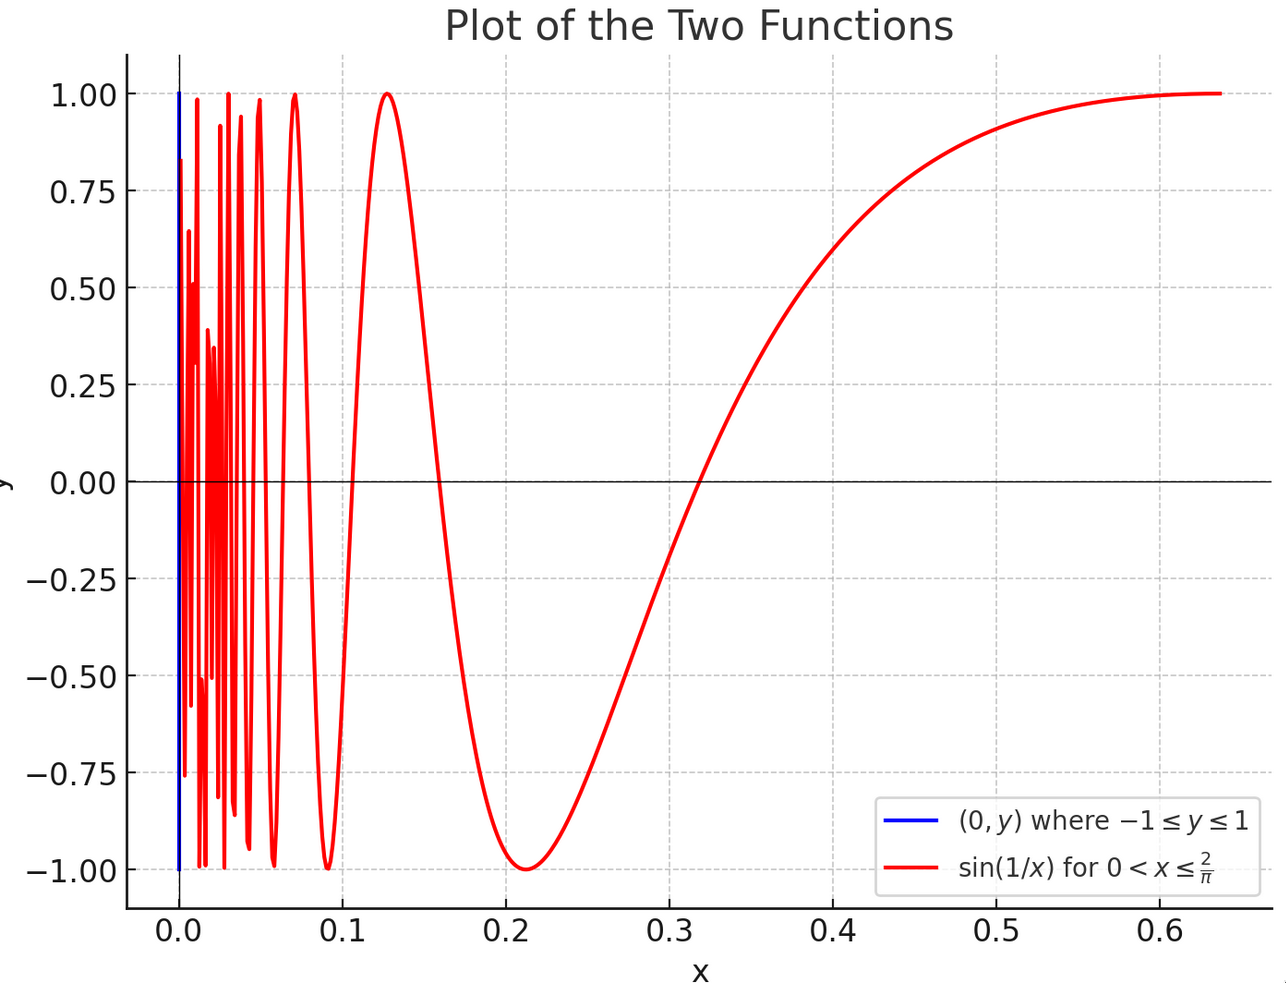
\includegraphics[width=0.8\textwidth]{assets/connected_set_example.png}
  \caption{$E$ is connected!}
  \label{fig:connected_set_example}
\end{figure}
Note that the red line never reaches the blue, so they don't intersect. \\
\end{note} 


\begin{theorem}
  Let $f:X \to Y$ a continous map and  $E \subseteq X$ (connected in  $X$) $\Rightarrow f(E)$ is connected in  $Y$.

  \begin{proof}
    Since $f:X \to Y$ is continuous, then  $f:E \to f(E)$ is also continuous. We are given that $\left( E,\rho \right) $ is connected. Consider the strongest case where $E =X$, so  $\left( X, \rho_X \right) $ is connected and $Y = f(X)$. Since by subspace topology, we can always restrict to $E \subseteq X, f:E \to f(E)$, then the above case is enough to prove the statement for all cases. \\


    Thus, we will prove that if $f:X \to Y$ is continuous and  $X$ is not connected and  $f(X) = Y$ then  $Y$ is connected. Prove this by contradiction, assume that the above holds but $Y$ is not connected. Then,
    \[
    Y = U \amalg V, U_{\text{open}} \neq \emptyset, V_{\text{open}} \neq \emptyset
    .\] 
    Consider the pre-images which we know are open due to continuous map theorems.
    \[
    f^{-1}\left( U \right) \subseteq X, f^{-1}\left( V \right) \subseteq X
    .\]
    We also know that both pre-images are not empty because the image is not empty and the map is onto (we construct $f(X) = Y$).
    \[
      f^{-1}\left( U \right) \neq \emptyset, f^{-1} \left( V \right)  \neq \emptyset
    .\]
    We can use the following result from set theory:
    \[
    f^{-1} \left( U \cap V \right) = f^{-1} (U) \cap f^{-1} (V)
    .\]
    And we know that $U \cap V = \emptyset$ because $U \amalg V$ (disjoint union), so
    \begin{align*}
      f^{-1} \left( U \cap V \right) &=    f^{-1} \left( \emptyset \right) \\
                                     &= \emptyset  \\
                                     &=  f^{-1} (U) \cap f^{-1} (V)
    .\end{align*}
    This means that open set $f^{-1}(U), f^{-1}(V)$ in $X$ and which $f^{-1}(U) \cup f^{-1}(V) = X$ and $f^{-1}(U) \cap f^{-1}(V) = \emptyset$, so $f^{-1}(U) \amalg f^{-1}(V) = X$ and $X$ is not connected. This is a contradiction. Thus,  if $f:X \to Y$ is continuous and  $X$ is not connected and  $f(X) = Y$ then  $Y$ is connected which is enough to prove the more general statement $f: X \to Y$ continuous map and  $E \subseteq X$  $\Rightarrow f(E)$ connected in  $Y$.
       
  \end{proof}
\end{theorem}

\subsection{connected sets in $\R$}
\begin{theorem}
  $E \subseteq \R$ is not connected $\iff$ $\exists x,y \in E,$ s.t. $ x < y$ and $x < z < y$, where  $z \not\in E$ 
  \begin{proof}
    $\left( \Rightarrow \right) $ Assume that $E$ is not connected. Then, $\exists U \neq \emptyset, V \neq \emptyset$, $U,V$ open in $E$,  $E = U \amalg V $ ($U = X \setminus V$ but $V$ is open, so $U$ is open and closed and by the same arugment  $V$ is also open and closed). Take $x \in U, y \in V$. Without loss of generality, assume that  $x < y$. Consider
     \[
       \alpha = sup\left( [x,y] \cap U \right) 
     .\]
     which must exist as $[x,y]$ is bounded and  $U$ is bounded. Consider the following cases:
      \begin{enumerate}
       \item If $\alpha \not\in E$ then  $x < \alpha < y$ (since  $x,y \in E$ and  $\alpha \not\in E$). The theorem thus holds for all $z = \alpha$
       \item   If $\alpha \in E$ then either:
         \begin{enumerate}
           \item $\alpha \in U$ then since $U$ is open in  $E$,  $\exists  \epsilon > 0$ such that \[
           B_\epsilon (\alpha)^{E} = (\left( \alpha - \epsilon, \alpha + \epsilon \right) \cap E) \subseteq U
           .\] and $\alpha + \epsilon < y$. Take $z \in \left( \alpha, \alpha + \epsilon \right) $,
           \begin{enumerate}
             \item If $z \not\in E$ then $x \leq \alpha < z < \alpha + \epsilon < y$. Hence, the theorem follows in this case
             \item   If $z \in E$, then  $z > \alpha$,  $e \in [x,y] \cap U \Rightarrow \alpha$ is not the $sup([x,y] \cap U)$  so this arugment is not possible. 
           \end{enumerate}
         \item If $\alpha \in V$ then this means that $\alpha \not\in ([x,y] \cap U)$. Then $\alpha$ is a limit point of  $[x,y] \cap U \Rightarrow$ $\alpha \in E$ is a limit point of $U$. Note that  $U$ is both open and closed in  $E$ which implies that $\alpha \in U$, but we know  $V \cap U = \emptyset$, so this is a contradiction!
         \end{enumerate}
     \end{enumerate}
  \end{proof}
\end{theorem}

\begin{definition}
  A subset $E$ is convex if  $\forall x,y \in E$ we have that  $[x,y] = \{tx + (1-t)y \mid 0 \leq t \leq 1\}  \subseteq E$ 
\end{definition}

\begin{theorem}
  $E \subseteq \R$ is connected $\iff E$ is convex. 
  
  \begin{proof}

  \end{proof}
\end{theorem}

\begin{corollary}
  A subset $E \subseteq \R$ is connected $\iff$ $E$ is one of the following sets:  \\
  $\emptyset, \R, (a,b), [a,b], [a,b), (a,b], (-\infty,a], (a, \infty), [a, \infty)$
\end{corollary}

\subsection{Intermediate Value Theorem}
\begin{corollary}
  If $f:[a,b] \to \R$ be continuous and $f(a) < f(b).$ Then if  $f(a) < c < f(b)$ then  $\exists x_{*} \in [a,b]$ such that $f(x_{*})  = c$. 

  \begin{proof}
    The interval $[a,b]$ is connected and compact  (in $[a,b]$, we restrict to $[a,b]$ because the function only defined as  $[a,b]$) then since $f:[a,b] \to \R$ is continuous, $f([a,b])$ must also be connected and compact in  $\R$ $\Rightarrow f([a,b]) = [A,B]$. Since the interval exists then $f(x_{*}) \in [A,B]$ exists and must be the image of $x_{*} \in [a,b]$. 

    \begin{note}
      We don't necessarily need compactness just to prove the above theorem, we use compactness for the stronger conclusion that the image of a closed interval under a continuous map is also a closed interval (where closed interval in $\R$ is connected and compact). 
    \end{note}
  \end{proof}
\end{corollary}

\section{Path Connected}
\begin{definition}
  $X$ is path connected if  $\forall x,y \in X$  $\exists $ a continuous map $\gamma [0,1] \to X$ such that  $\gamma(0) = x, \gamma(1) =y$.
\end{definition}

\begin{prop}
  If $(X,\rho)$ is path connected  $\Rightarrow$  $X$ is connected i.e.  $\{\text{path connected sets}\} \subseteq \{\text{connected sets}\}  $
\end{prop}

\end{document}
